The experiments were conducted as follows. Training consisted of nine example grasps, executed in simulation, with a human in control. These nine grasps were grouped into three grasp types (rim, pinch, and handle). The rim and pinch grasp types were trained on the colander object, and the handle grasp type was demonstrated on the saucepan. During testing an object was placed on the table. Every grasp type was compared automatically, and one selected for execution according to the methods described above. The models of the test objects consisted of a point cloud taken from just one view. Thus reconstructions were partial, typically less that 25\% of the object's surface area. No test objects had been seen previously by the robot, and it can be seen from Fig.~\ref{fig:test}. Fifteen test objects were presented, and 12 of the 15 test grasps succeeded, giving a generalisation success rate of 80\%. While the difference is not statistically significant, this is slightly higher than the 77.7\% success rate we recorded on a larger test set for a fully actuated hand also working from a single view of an object \cite{kopicki-ijrr15}.

\begin{figure}
 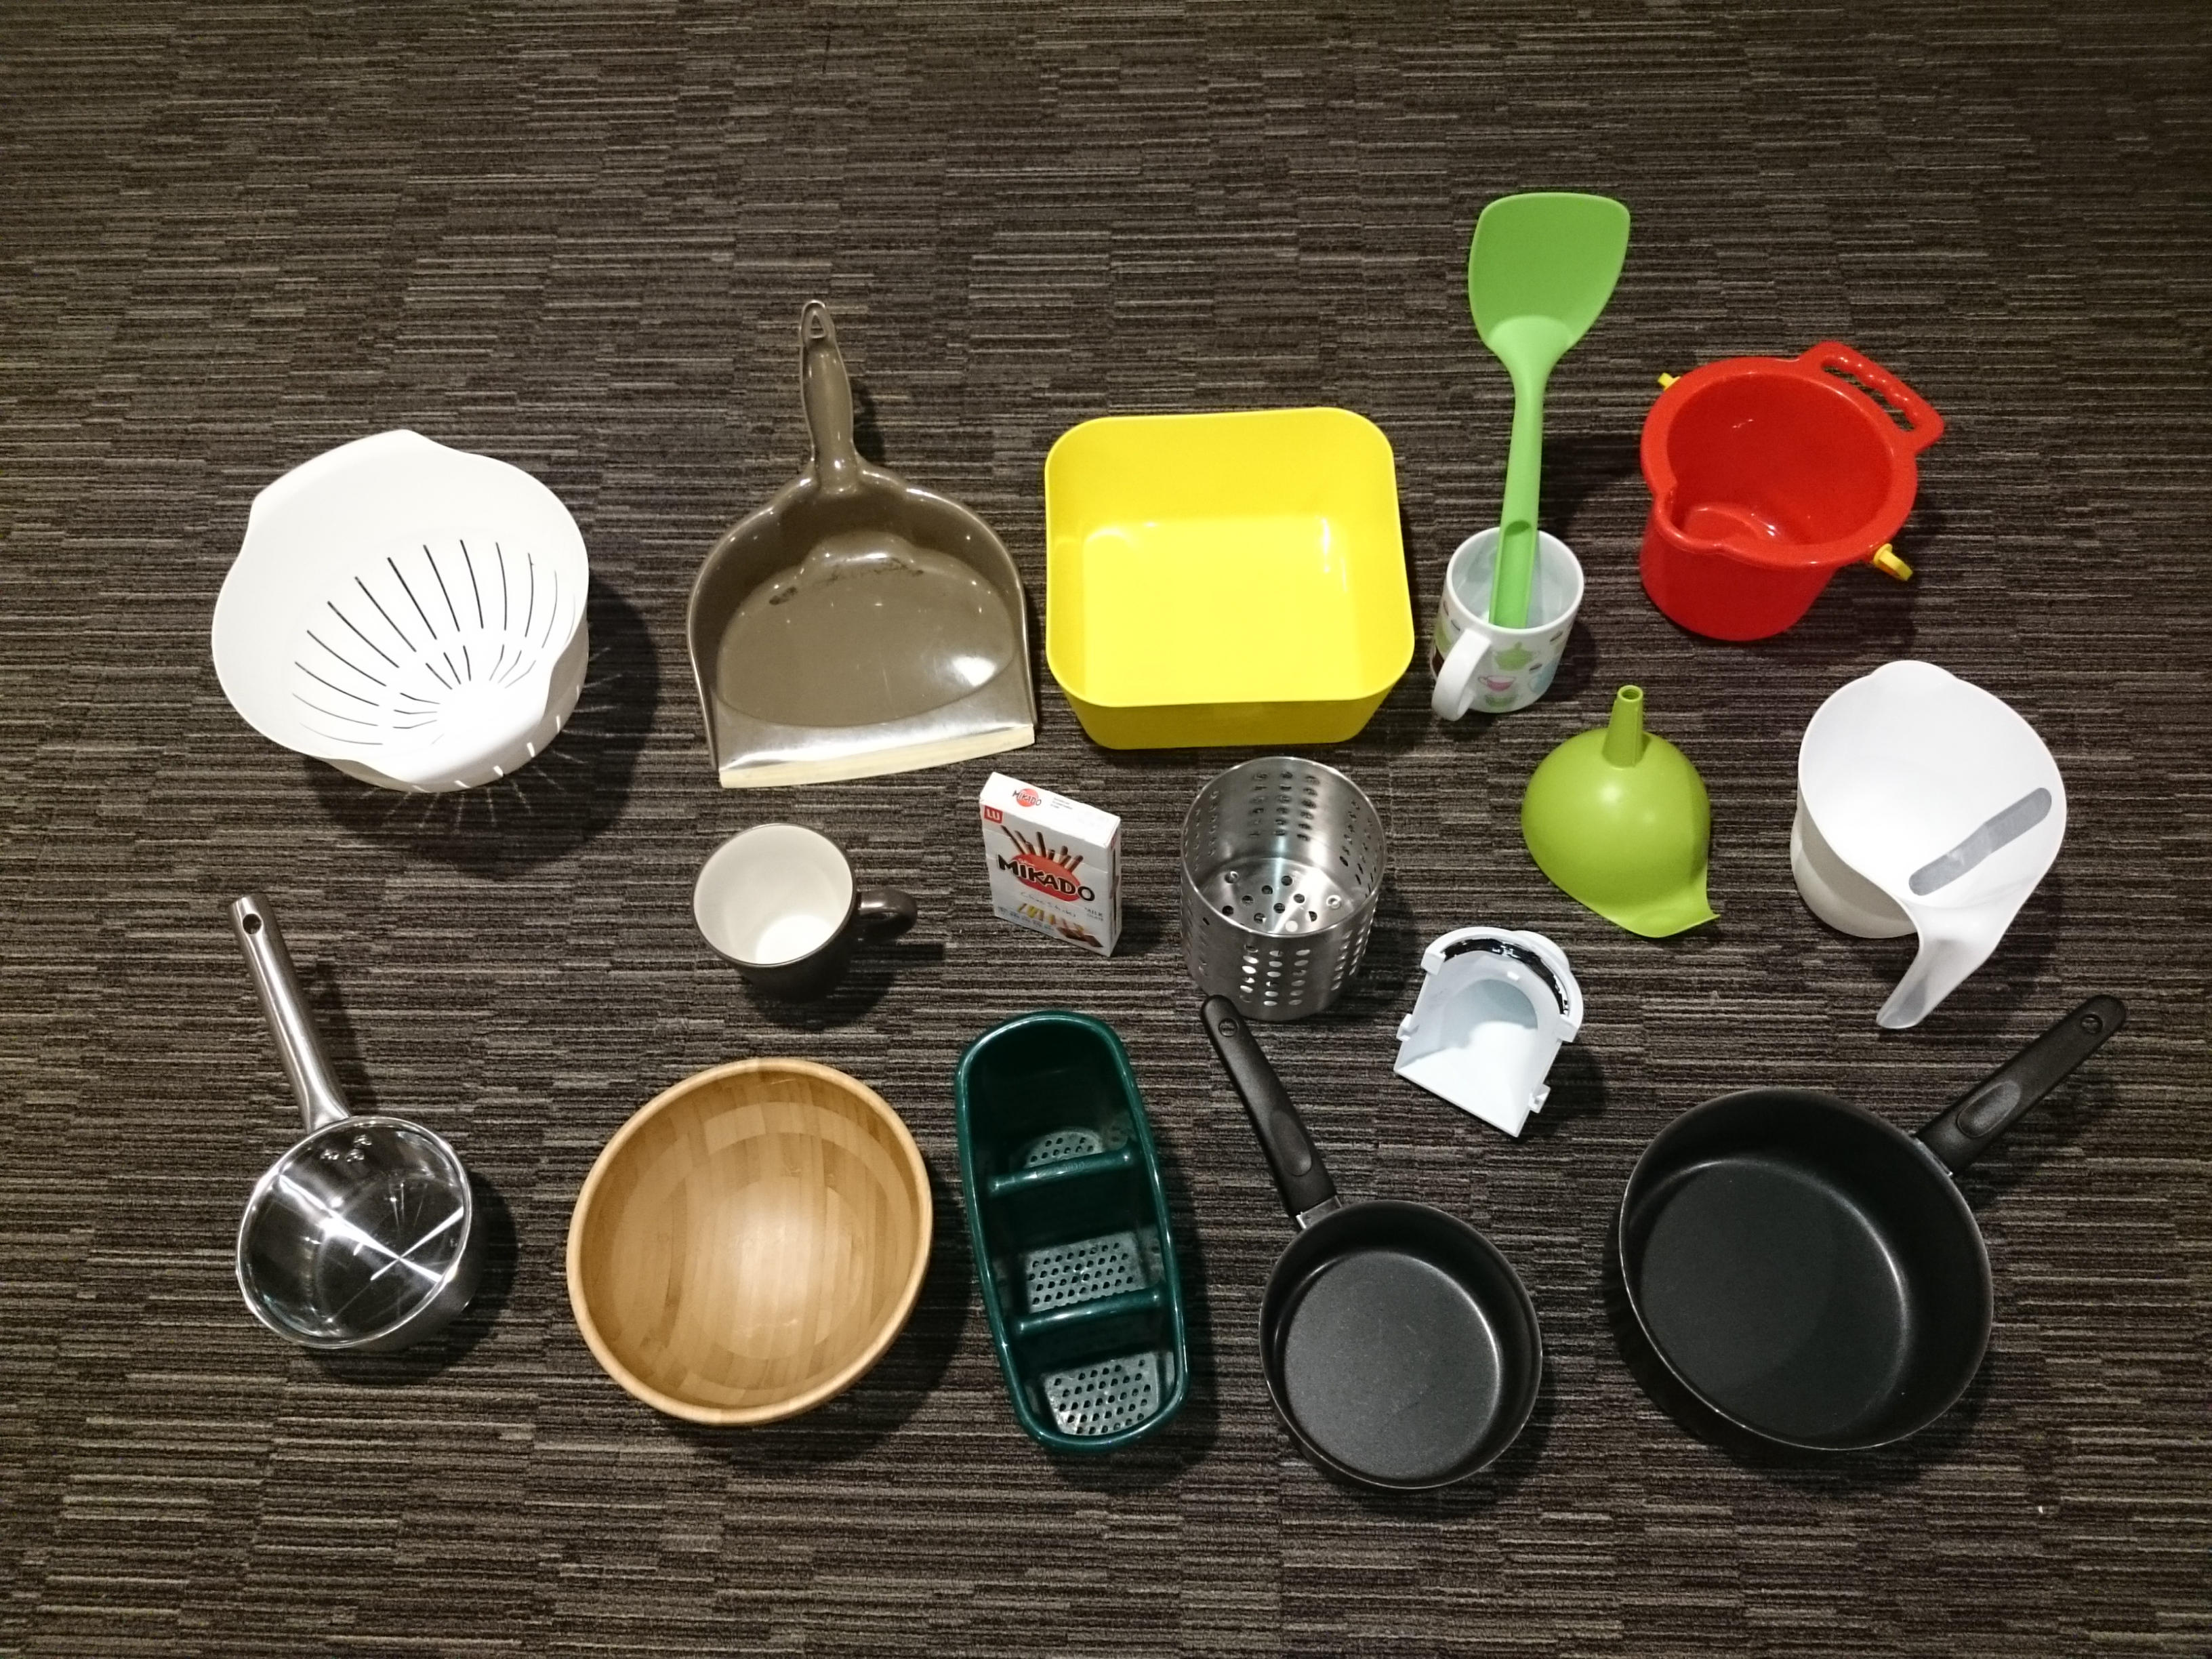
\includegraphics[width=0.9\columnwidth]{images/object_set}
 \caption{The two training objects are on the far left. The testing objects on the right. 12 from 15 test grasps on novel objects were successful.}
 \label{fig:test}
\end{figure}

\begin{figure*}
\begin{center}
\newcommand{\tw}{0.15\linewidth}
 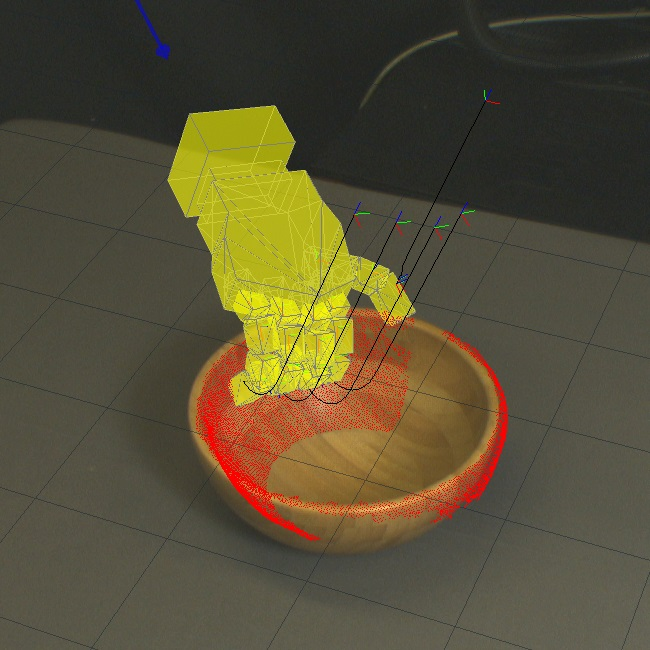
\includegraphics[width=\tw]{images/experiments/query/bowllarge-1-s}
 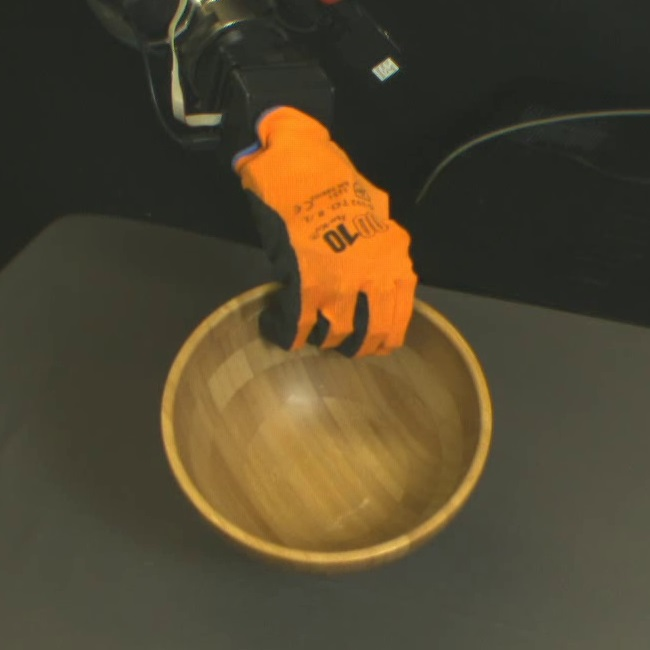
\includegraphics[width=\tw]{images/experiments/exec/bowllarge-s}
 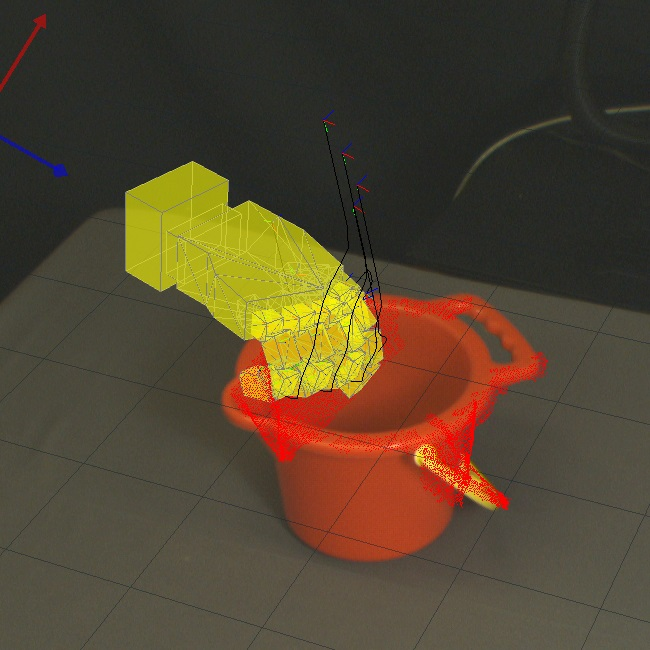
\includegraphics[width=\tw]{images/experiments/query/bucket-1-s}
 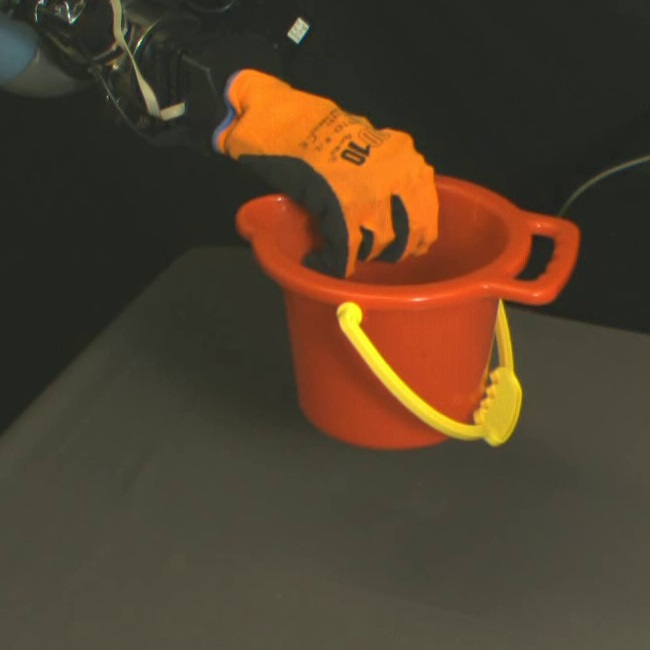
\includegraphics[width=\tw]{images/experiments/exec/bucket-s}
  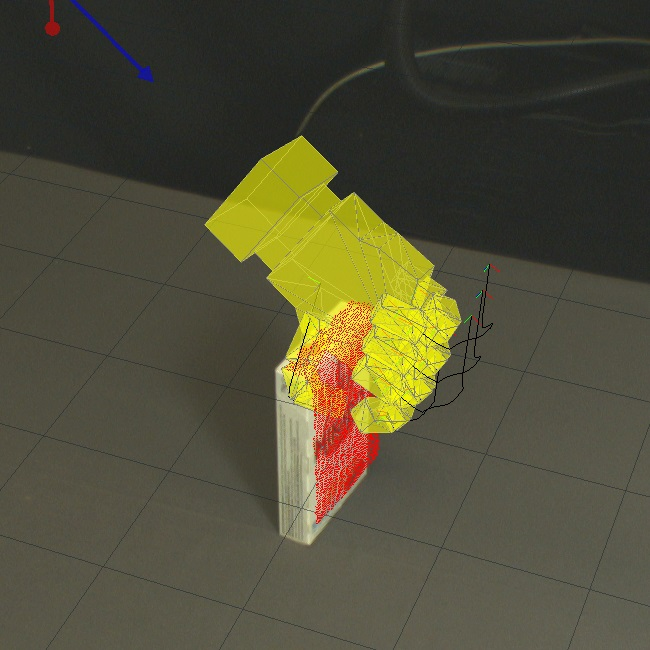
\includegraphics[width=\tw]{images/experiments/query/chocsticks-1-s}
 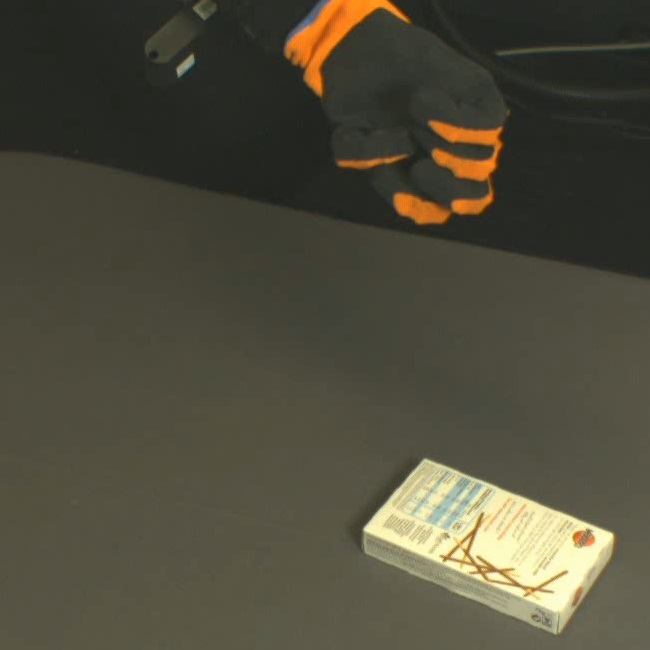
\includegraphics[width=\tw]{images/experiments/exec/chocsticks-s}\\
  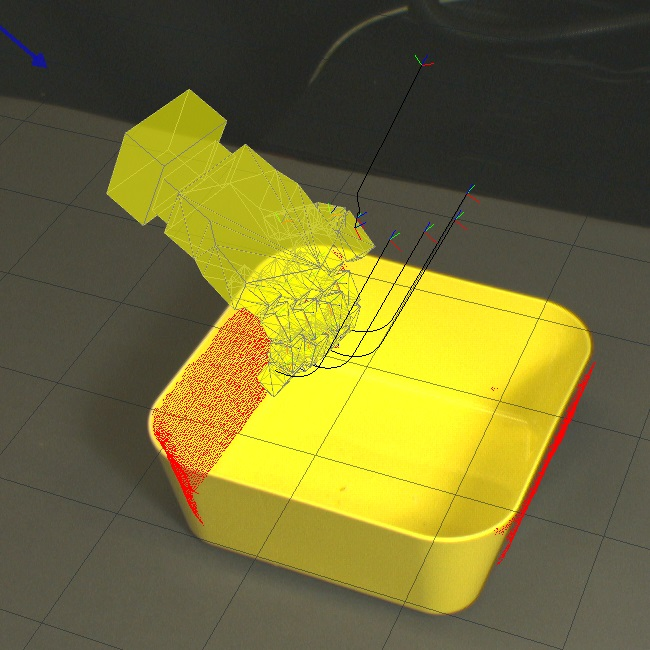
\includegraphics[width=\tw]{images/experiments/query/container1-1-s}
 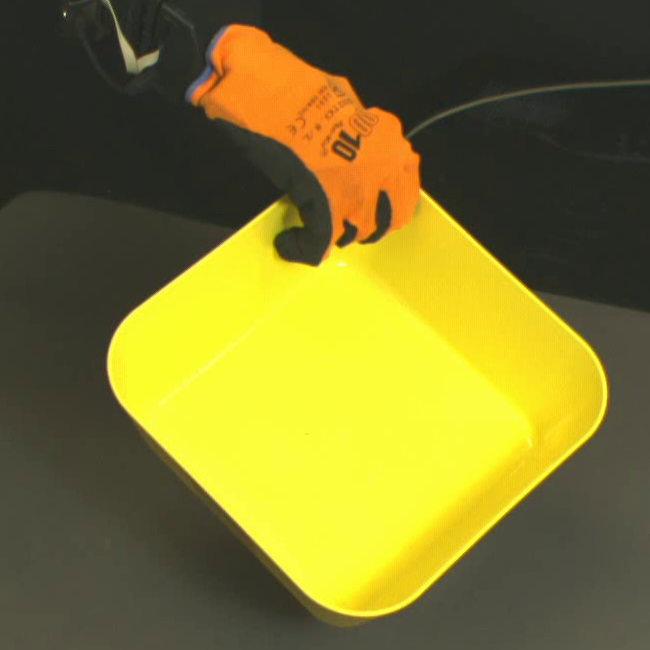
\includegraphics[width=\tw]{images/experiments/exec/container1-s}
  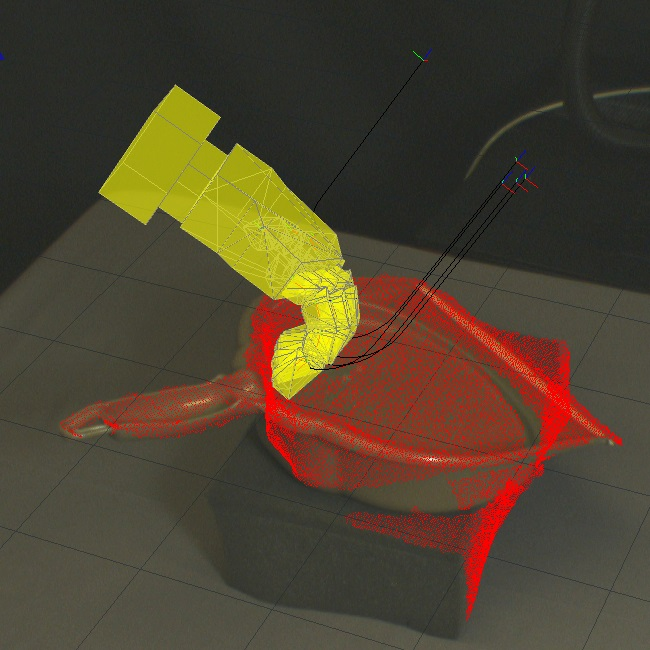
\includegraphics[width=\tw]{images/experiments/query/dustpan-1-s}
 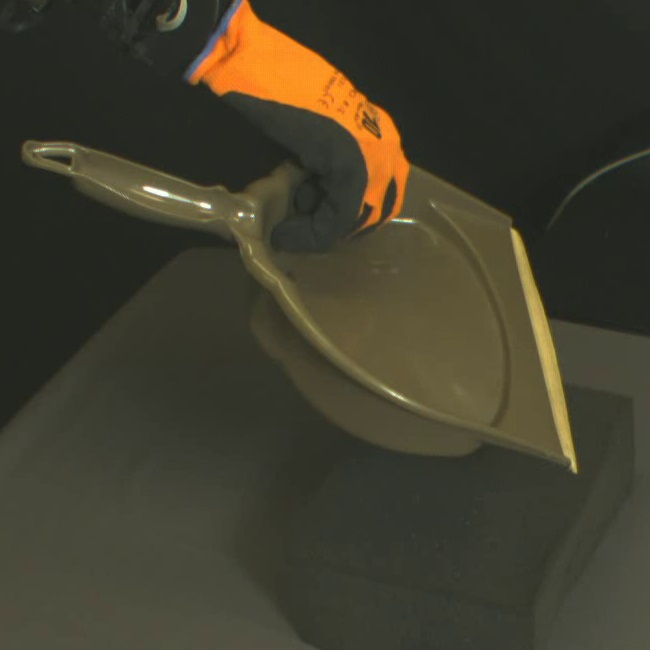
\includegraphics[width=\tw]{images/experiments/exec/dustpan-s}
  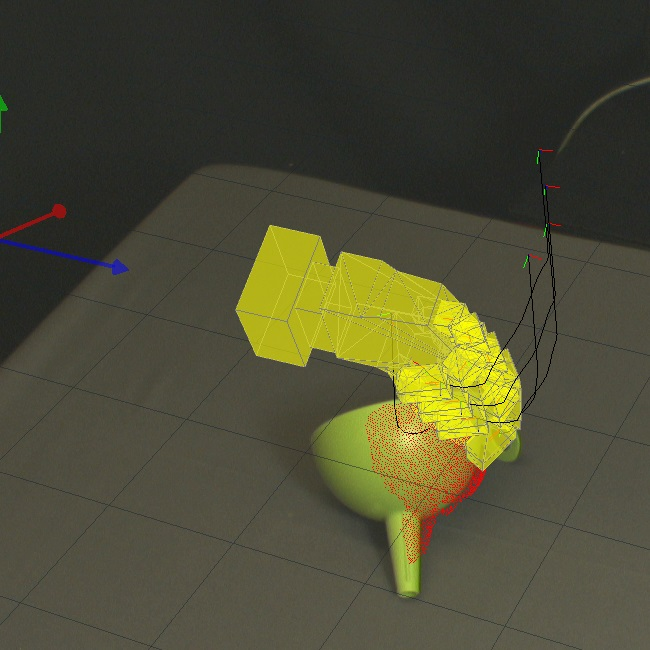
\includegraphics[width=\tw]{images/experiments/query/funnellarge-1-s}
 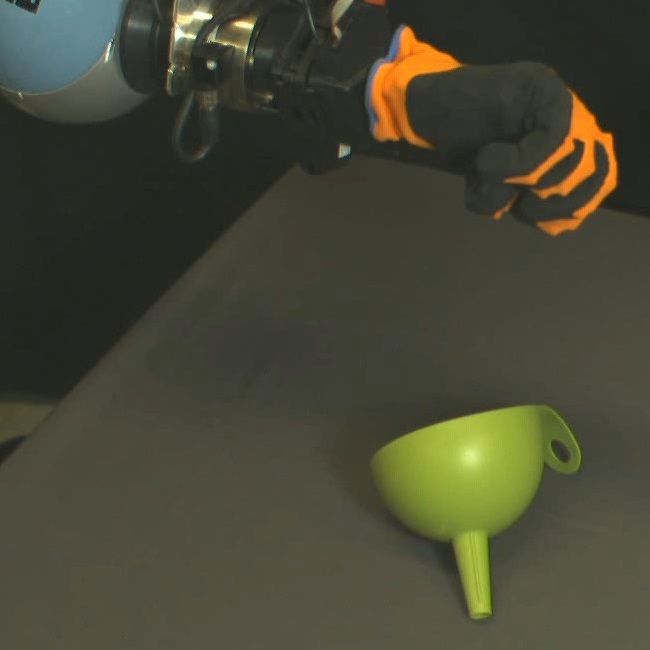
\includegraphics[width=\tw]{images/experiments/exec/funnellarge-s}\\
  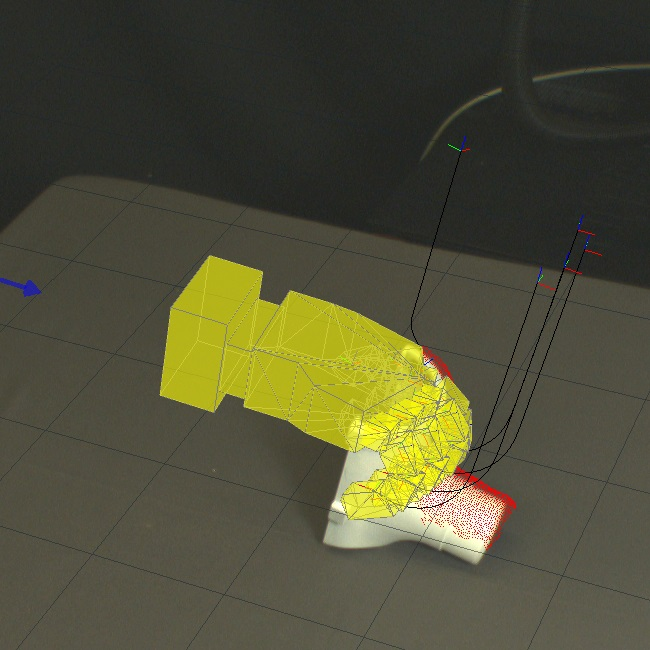
\includegraphics[width=\tw]{images/experiments/query/guttering-1-s}
 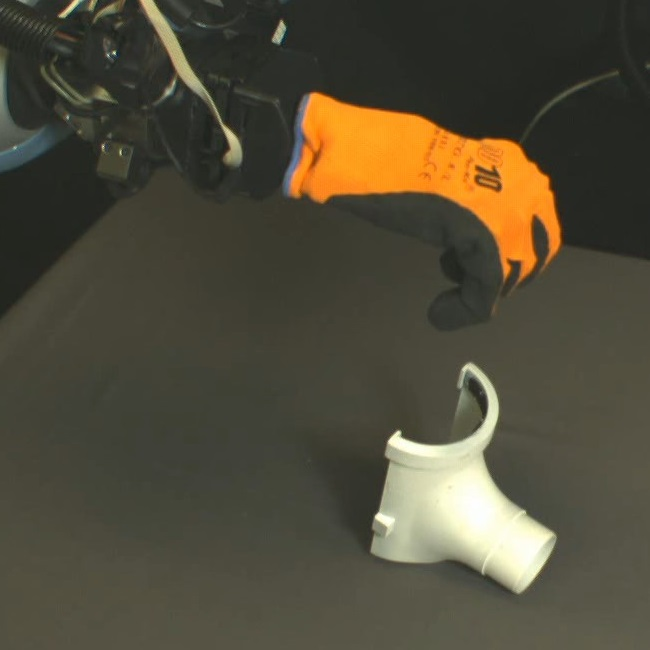
\includegraphics[width=\tw]{images/experiments/exec/guttering-s}
  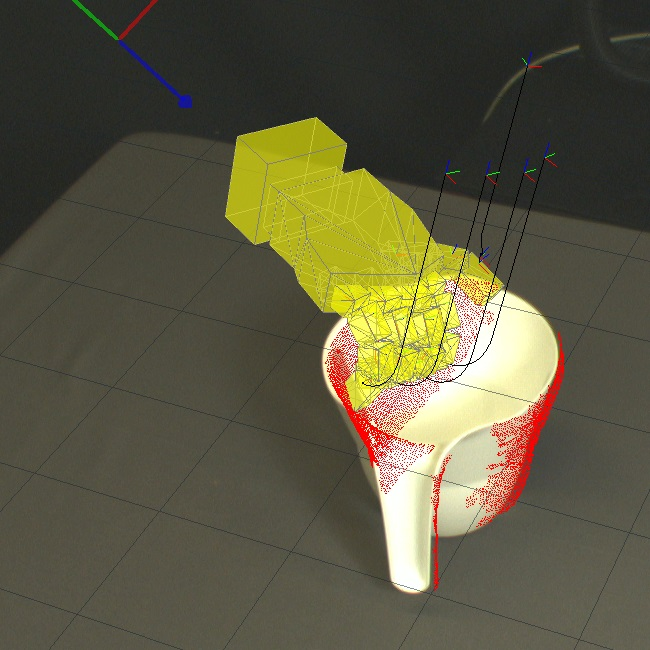
\includegraphics[width=\tw]{images/experiments/query/jug-1-s}
 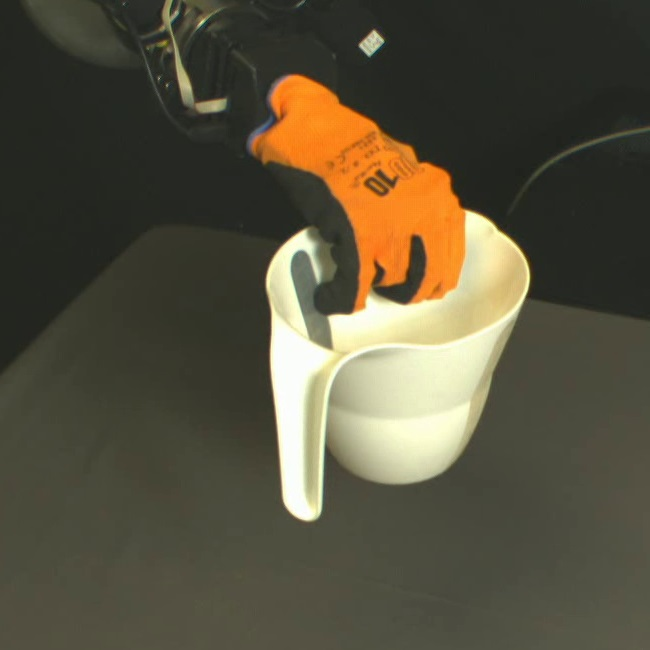
\includegraphics[width=\tw]{images/experiments/exec/jug-s}
  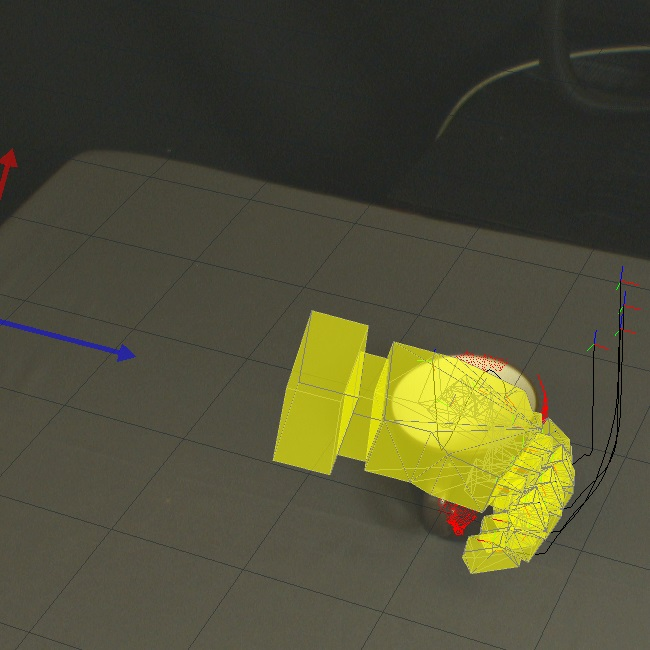
\includegraphics[width=\tw]{images/experiments/query/mug1-1-s}
 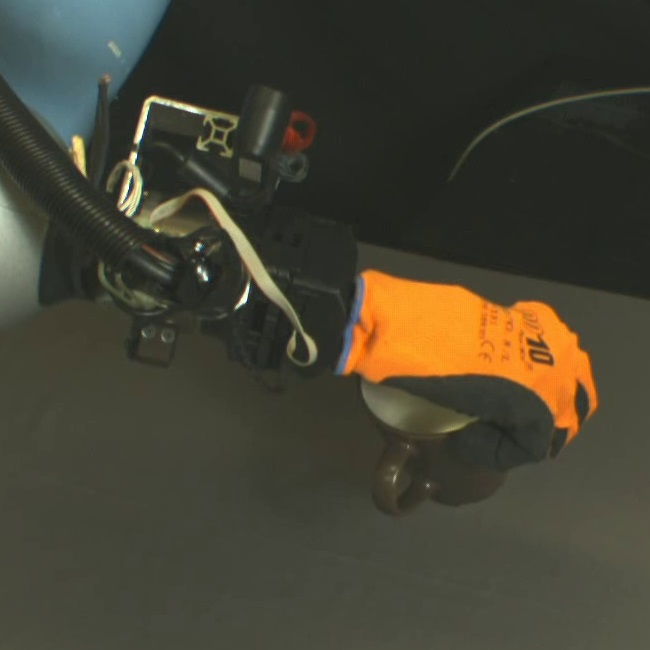
\includegraphics[width=\tw]{images/experiments/exec/mug1-s}\\
  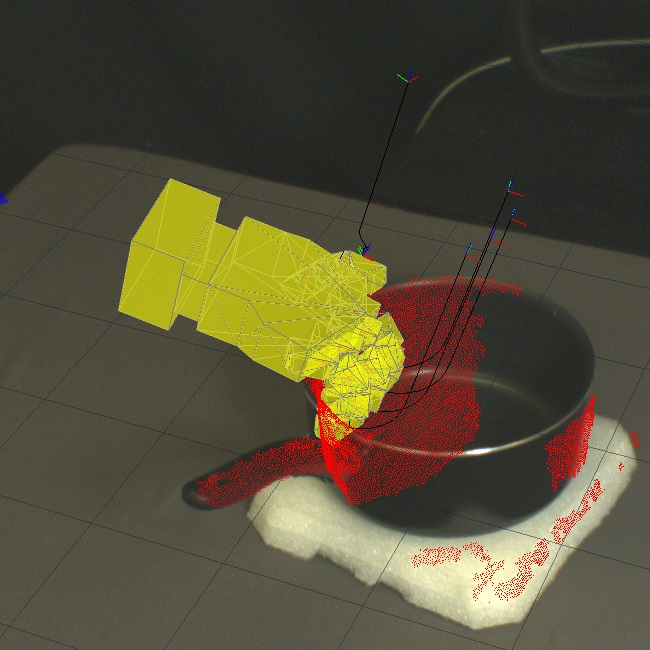
\includegraphics[width=\tw]{images/experiments/query/saucepanlarge-1-s}
 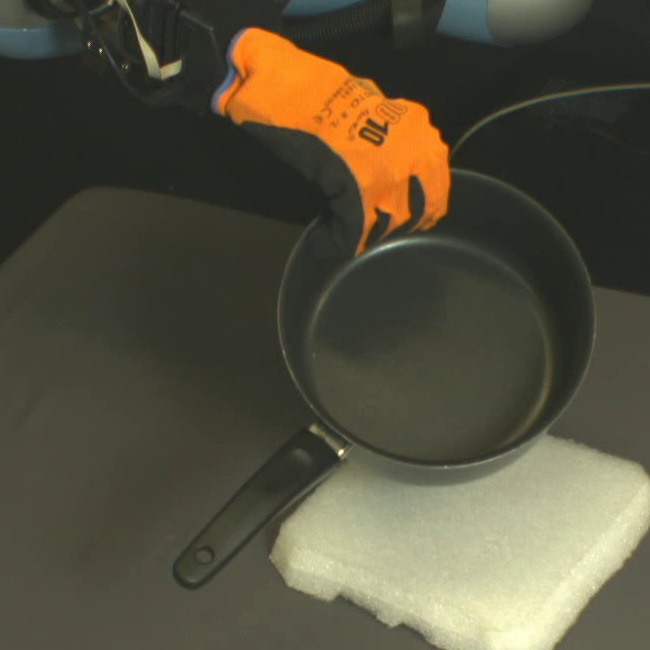
\includegraphics[width=\tw]{images/experiments/exec/saucepanlarge-s}
  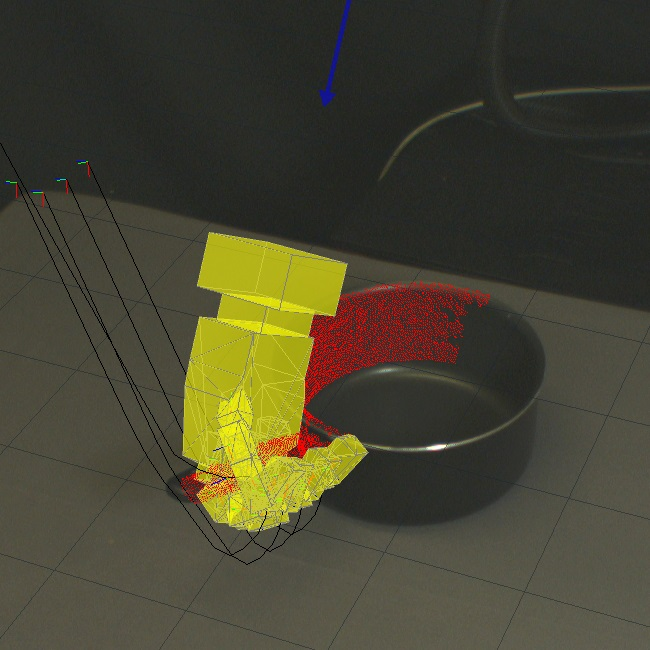
\includegraphics[width=\tw]{images/experiments/query/saucepanlarge-handle-1-s}
 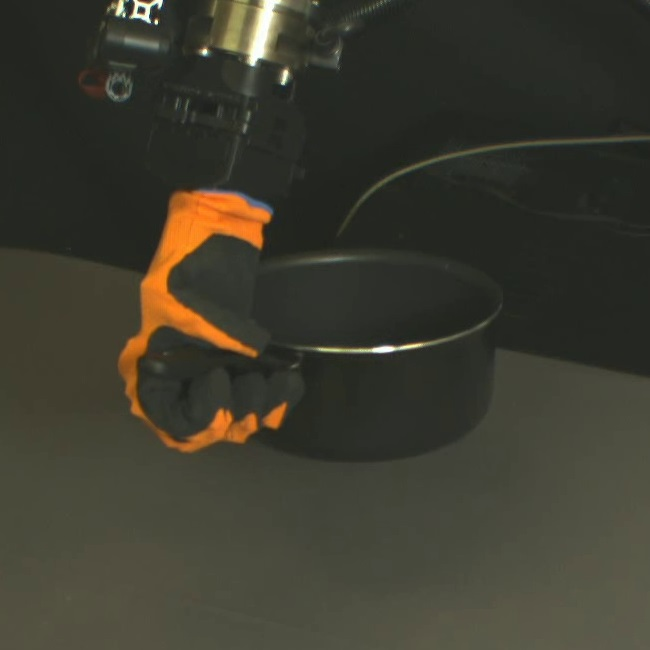
\includegraphics[width=\tw]{images/experiments/exec/saucepanlarge-handle-s}
  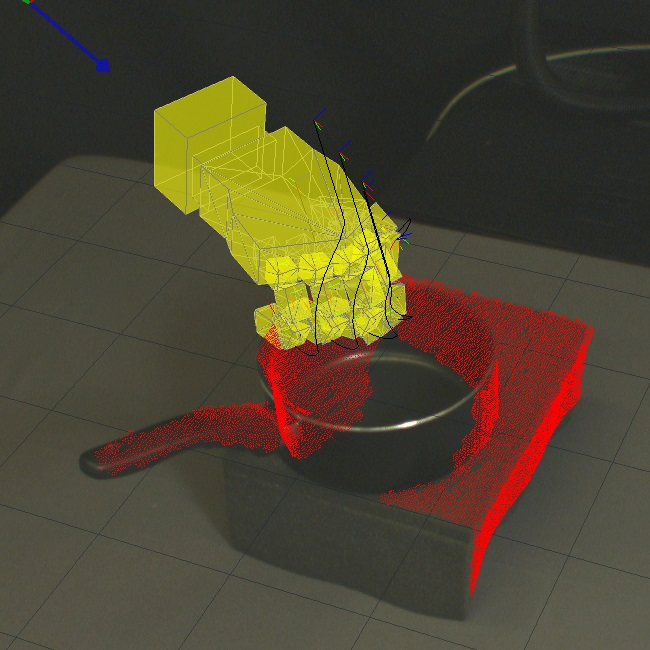
\includegraphics[width=\tw]{images/experiments/query/saucepansmall-1-s}
 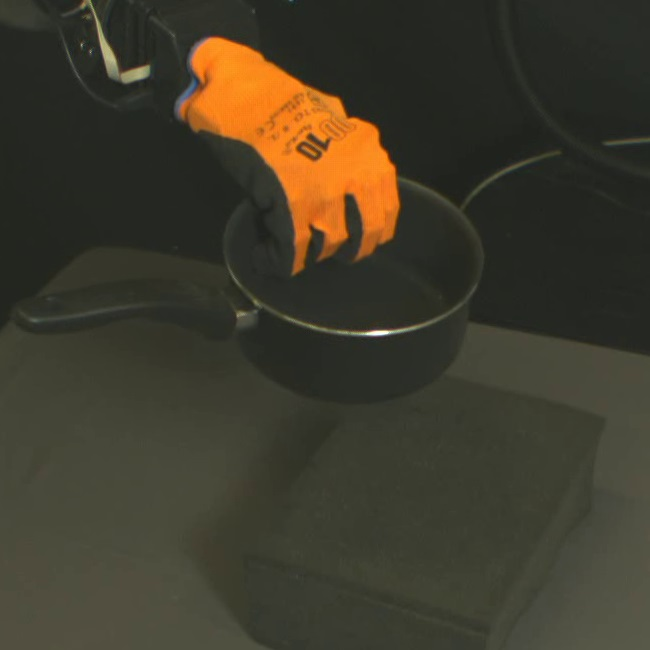
\includegraphics[width=\tw]{images/experiments/exec/saucepansmall-s}\\
  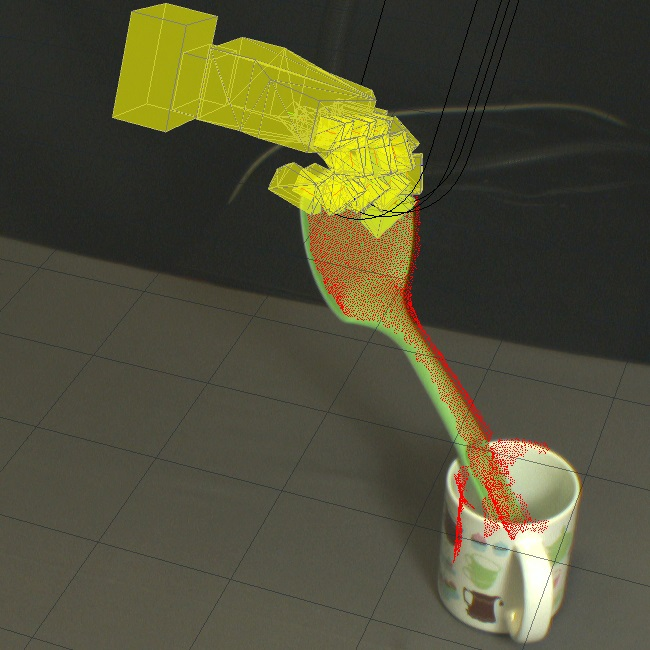
\includegraphics[width=\tw]{images/experiments/query/spatula-1-s}
 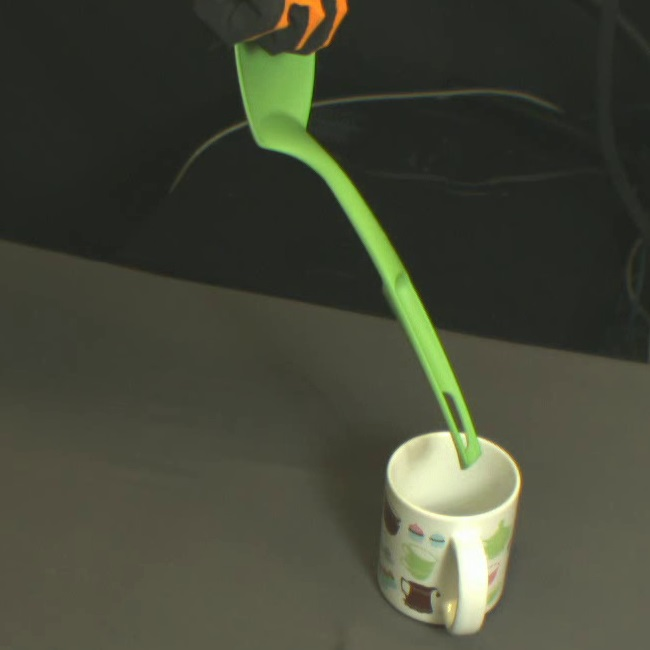
\includegraphics[width=\tw]{images/experiments/exec/spatula-s}
  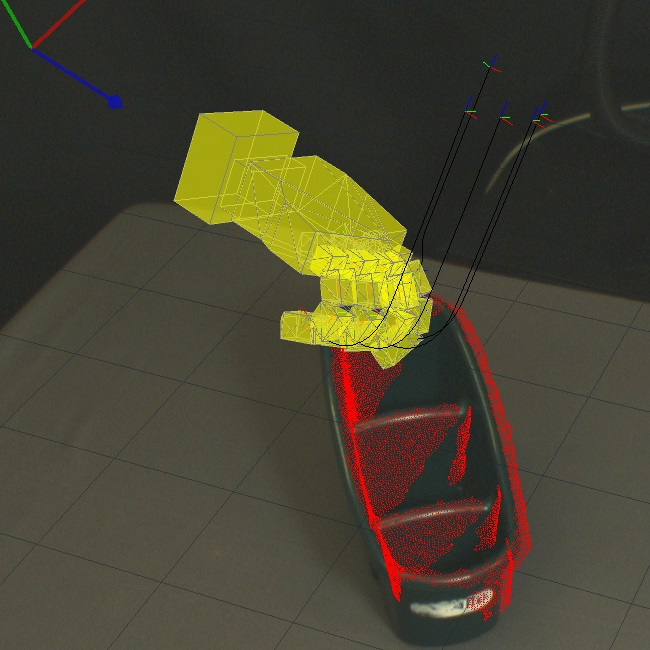
\includegraphics[width=\tw]{images/experiments/query/stand1-1-s}
 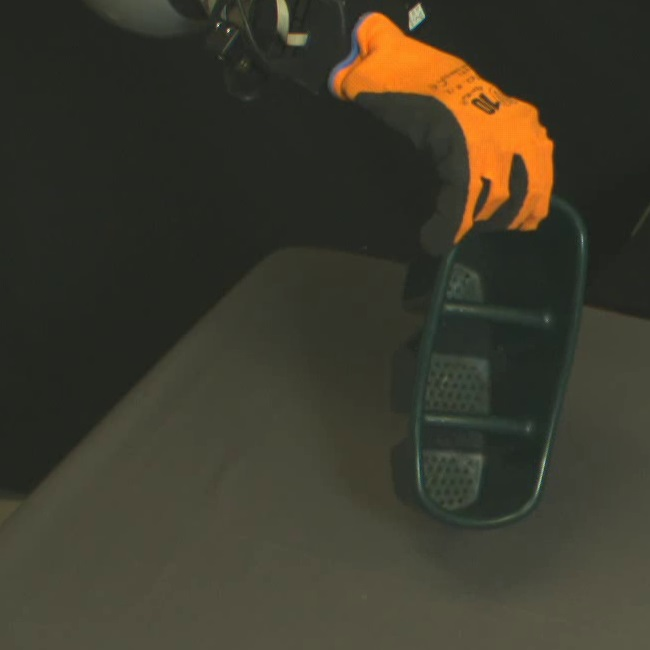
\includegraphics[width=\tw]{images/experiments/exec/stand1-s}
  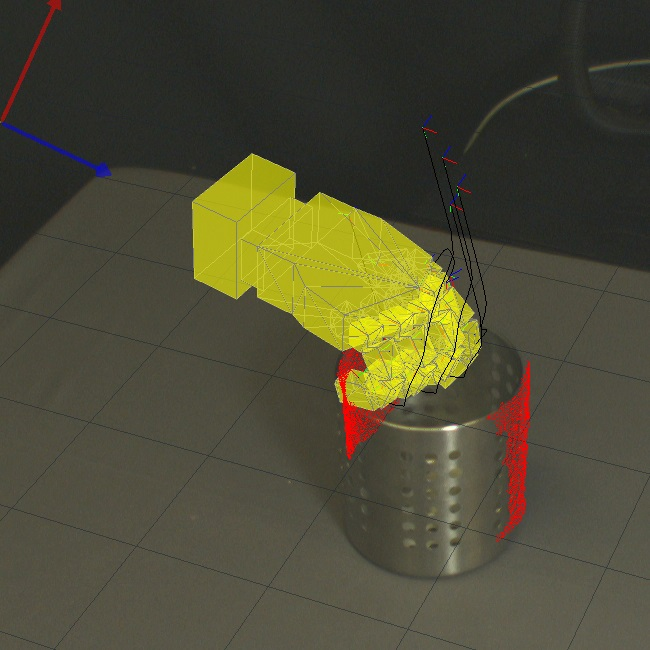
\includegraphics[width=\tw]{images/experiments/query/stand2-1-s}
 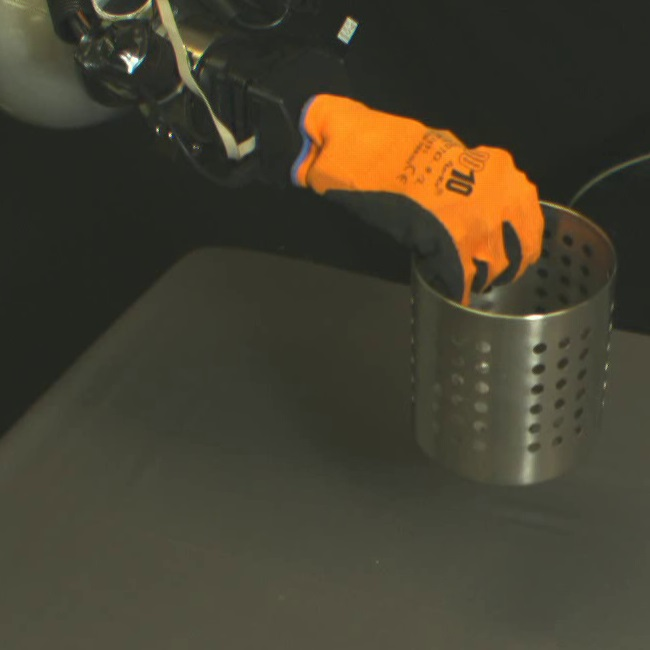
\includegraphics[width=\tw]{images/experiments/exec/stand2-s}
 \caption{The fifteen test grasps. Each one has a pair of images. The predicted equilibrium grasp state is shown on the left of each pair, and the actual grasp on the right. Counting from top left it can be seen that grasps 3,6, and 7 failed. All other grasps succeeded.}
 \label{fig:test}
 \end{center}
\end{figure*}
